% ClearEval MICCAI 2026 main conference submission (LNCS format)
% This file is designed to compile out-of-the-box on Overleaf.
% It follows the provided "MICCAI2026-main conference paper template.tex".

\documentclass[runningheads]{llncs}

\usepackage[T1]{fontenc}
\usepackage{graphicx,verbatim}
\usepackage{amsmath,amssymb}
\usepackage{booktabs}
\usepackage{multirow}
\usepackage{url}
\usepackage[UTF8]{ctex} % 新增：为了支持中文字符的编译

\begin{document}

\title{ClearEval: A Data-driven physical grounding Benchmark
for the Design of Tissue Optical Clearing Protocols with Large Language Models\\
\vspace{0.5cm} \large ClearEval：用于大型语言模型设计组织光透明协议的数据驱动物理接地基准测试}
\titlerunning{ClearEval: Physics-Informed Benchmark for TOC}
%\titlerunning{ClearEval}

\begin{comment}  %% Removed for anonymized MICCAI submission
\author{First Author\inst{1}\orcidID{0000-1111-2222-3333} \and
Second Author\inst{2,3}\orcidID{1111-2222-3333-4444} \and
Third Author\inst{3}\orcidID{2222--3333-4444-5555}}
\authorrunning{F. Author et al.}
\institute{University A \and University B \email{author@institute.edu}}
\end{comment}

% NOTE: Do not remove this anonymized author section for initial submission.
\author{Anonymized Authors}
\authorrunning{Anonymized Author et al.}
\institute{Anonymized Affiliations \\
    \email{email@anonymized.com}}

\maketitle

\begin{abstract}
Tissue optical clearing imaging enables the visualization of structural and functional information from a spatial perspective, offering new avenues to explore the essence of life. Tissue Optical Clearing (TOC) is the critical link for achieving this transparency, and the protocol design is a complex process. The protocol’s parameter misjudgments risk irreversible sample damage, which is strictly unacceptable for human pathological samples. While Large Language Models (LLMs) excel in biomedical knowledge retrieval, their capacity to generate actionable, physically feasible wet-lab protocols remains under-evaluated. Here, we propose the first expert-level benchmark dedicated to TOC protocol design (ClearEval). Based on curated literature and expert cases, we establish a comprehensive evaluation framework to assess both domain knowledge mastery and practical protocol generation capabilities. Beyond pure semantic metrics, we develop a multi-dimensional evaluation pipeline: an LLM-based structured evaluation for Completeness and Correctness, coupled with an empirically-grounded evaluation system for Effectiveness. The results reveal that while state-of-the-art models achieve over 85\% accuracy on static knowledge, their performance degrades significantly in generating physically-compliant protocols, exposing a substantial ``knowledge-action gap''. This work provides a rigorous pre-deployment gatekeeper for scientific agents, paving the way for autonomous, closed-loop 3D biomedical imaging workflows in the AI4Science era. The dataset and code are publicly available.

组织光透明成像能够从空间角度可视化结构和功能信息，为探索生命本质提供了新的途径。组织光透明（TOC）是实现这种透明化的关键环节，而协议设计是一个复杂的过程。协议参数的误判有对样本造成不可逆损伤的风险，这对于人类病理样本来说是绝对不可接受的。尽管大型语言模型（LLM）在生物医学知识检索方面表现出色，但它们生成可执行、物理上可行的湿实验协议的能力仍然缺乏评估。在此，我们提出了首个专门针对 TOC 协议设计的专家级基准测试（ClearEval）。基于精选的文献和专家案例，我们建立了一个全面的评估框架，以评估领域知识的掌握程度和实际协议的生成能力。除了纯粹的语义指标外，我们开发了一个多维评估管道：基于 LLM 的结构化评估（针对完整性和正确性），以及基于经验的有效性评估系统。结果表明，尽管最先进的模型在静态知识上达到了 85\% 以上的准确率，但它们在生成符合物理规律的协议时性能显著下降，暴露了巨大的“知行鸿沟”。这项工作为科学智能体提供了一个严格的部署前守门员，为 AI4Science 时代自主的、闭环的 3D 生物医学成像工作流铺平了道路。数据集和代码已公开。

\keywords{Benchmark \and Tissue optical clearing \and Wet-lab protocols \and Large language models \and Empirically-grounded evaluation}
\end{abstract}

\section{Introduction (引言)}

Tissue Optical Clearing (TOC) homogenizes the refractive indices of cellular components to render biological tissues transparent. This enables non-destructive, sub-cellular 3D imaging via light-sheet microscopy~\cite{ueda2020tissue,chung2013clarity}, preserving critical long-range 3D connectivity essential for constructing high-fidelity organ atlases. However, TOC protocol design is a complex multi-objective optimization problem where parameter misjudgments can lead to irreversible specimen damage.

组织光透明（TOC）通过均匀化细胞成分的折射率使生物组织变得透明。这使得通过光片显微镜进行非破坏性、亚细胞分辨率的 3D 成像成为可能~\cite{ueda2020tissue,chung2013clarity}，从而保留了构建高保真器官图谱所必需的关键长程 3D 连接。然而，TOC 协议设计是一个复杂的多目标优化问题，参数误判可能导致不可逆的标本损坏。

While Large Language Models (LLMs) demonstrate proficiency in biomedical question answering~\cite{singhal2023medpalm}, their capacity to synthesize actionable wet-lab protocols remains limited. Existing scientific benchmarks (e.g., MedQA~\cite{jin2021disease}, MMLU~\cite{hendrycks2021mmlu}) predominantly assess static knowledge recall. Furthermore, traditional semantic metrics (e.g., BLEU~\cite{papineni2002bleu}) and general-purpose ``LLM-as-a-judge'' evaluators~\cite{liu2023geval} fail to capture functional executability. A generated protocol with high linguistic similarity to a reference can still be experimentally invalid due to incorrect chemical concentrations. These generic evaluators lack the domain-specific physics grounding necessary to detect subtle wet-lab failures, often propagating hallucinations~\cite{bang2025hallulens}. Therefore, evaluating LLMs requires shifting from text-based similarity to rigorous protocol planning under physical constraints.

尽管大型语言模型（LLM）在生物医学问答中表现出熟练度~\cite{singhal2023medpalm}，但它们合成可操作的湿实验协议的能力仍然有限。现有的科学基准测试（如 MedQA~\cite{jin2021disease}，MMLU~\cite{hendrycks2021mmlu}）主要评估静态知识的回忆。此外，传统的语义指标（如 BLEU~\cite{papineni2002bleu}）和通用的“LLM作为裁判”评估器~\cite{liu2023geval}未能捕捉功能上的可执行性。一个与参考文本具有高语言相似度的生成协议，由于化学浓度错误，在实验中仍然可能是无效的。这些通用评估器缺乏检测微妙湿实验失败所需的特定领域物理基础，常常导致幻觉的传播~\cite{bang2025hallulens}。因此，评估 LLM 需要从基于文本的相似性转向在物理约束下严谨的协议规划。

To bridge this gap, we introduce \textbf{ClearEval}, the first benchmark dedicated to wet-lab grounded TOC protocol design. Distinct from purely textual evaluations, ClearEval integrates an empirically-grounded evaluation pipeline based on a comprehensive expert taxonomy. We propose the \textbf{CCE (Completeness, Correctness, Effectiveness) framework}, which rigorously validates generated protocols against empirical wet-lab constraints and experimental confidence intervals, rather than relying on static reference texts. Our main contributions are: 
(1) The first wet-lab grounded TOC benchmark for evaluating functional executability; 
(2) A curated dataset of 2,589 MCQs and 253 physics-constrained protocol design tasks; 
(3) The CCE framework, which quantitatively measures the LLM performance gap in practical experimental planning.

为了弥合这一鸿沟，我们引入了 \textbf{ClearEval}，这是首个致力于湿实验落地的 TOC 协议设计基准测试。与纯文本评估不同，ClearEval 基于全面的专家分类法，集成了一个基于经验事实的评估管道。我们提出了 \textbf{CCE（完整性、正确性、有效性）框架}，该框架根据经验性的湿实验约束和实验置信区间严格验证生成的协议，而不是依赖静态的参考文本。我们的主要贡献是：
(1) 首个基于湿实验的 TOC 基准测试，用于评估功能可执行性；
(2) 一个包含 2,589 个选择题（MCQ）和 253 个受物理约束的协议设计任务的精选数据集；
(3) CCE 框架，它定量衡量了 LLM 在实际实验规划中的性能差距。

\section{Related Work (相关工作)}
\subsection{LLMs in Biomedicine and Scientific Agents (生物医学和科学智能体中的 LLM)}

While LLMs demonstrate expert-level performance on static biomedical benchmarks (e.g., MedQA~\cite{jin2021disease}, PubMedQA~\cite{jin2019pubmedqa}, MMLU-Pro~\cite{wang2024mmlupro}), these tasks predominantly evaluate declarative knowledge retrieval rather than procedural wet-lab synthesis. Recent domain-specific benchmarks like ChemBench~\cite{mirza2025chembench} and CSEDB~\cite{wang2025csedb} highlight the limitations of general models in specialized scientific problem-solving. Moving beyond static QA, scientific agents (e.g., ChemCrow~\cite{bran2024chemcrow}, Coscientist~\cite{boiko2024autonomous}) integrate LLMs with robotic execution for chemical synthesis. However, wet-lab tissue preparation like TOC involves complex spatiotemporal diffusion within heterogeneous tissues, lacking the strict stoichiometry of chemistry or the virtual sandbox of bio-coding~\cite{odonoghue2023bioplanner}. Current agents lack the physical grounding to safely navigate these continuous-variable spaces.

尽管 LLM 在静态生物医学基准测试（例如 MedQA~\cite{jin2021disease}、PubMedQA~\cite{jin2019pubmedqa}、MMLU-Pro~\cite{wang2024mmlupro}）上表现出专家级性能，但这些任务主要评估陈述性知识的检索，而不是程序性的湿实验合成。最近的特定领域基准测试（如 ChemBench~\cite{mirza2025chembench} 和 CSEDB~\cite{wang2025csedb}）突显了通用模型在专业科学问题解决中的局限性。超越静态问答，科学智能体（如 ChemCrow~\cite{bran2024chemcrow}、Coscientist~\cite{boiko2024autonomous}）将 LLM 与机器人执行结合用于化学合成。然而，像 TOC 这样的湿实验组织制备涉及异质组织内复杂的时空扩散，缺乏化学严格的化学计量或生物编码的虚拟沙盒~\cite{odonoghue2023bioplanner}。当前的智能体缺乏安全导航这些连续变量空间所需的物理接地。

\subsection{Limits of Semantic Evaluation (语义评估的局限性)}

Traditional metrics (e.g., BLEU~\cite{papineni2002bleu}) and general-purpose LLM-as-a-judge evaluators~\cite{liu2023geval} often fail to assess the functional executability of scientific protocols, suffering from ``hallucination resonance'' where subtle physical violations go undetected~\cite{bang2025hallulens}. ClearEval addresses this by introducing an empirically-grounded evaluator, anchoring assessment in deterministic physical laws and chemical constraints, ensuring high scores reflect genuine wet-lab viability.

传统指标（如 BLEU~\cite{papineni2002bleu}）和通用的“LLM作为裁判”评估器~\cite{liu2023geval}通常无法评估科学协议的功能可执行性，容易遭受“幻觉共鸣”的困扰，即微妙的物理违规行为未被检测到~\cite{bang2025hallulens}。ClearEval 通过引入基于经验事实的评估器解决了这一问题，将评估锚定在确定性的物理定律和化学约束上，确保高分反映真实的湿实验可行性。

\section{The ClearEval Benchmark (ClearEval 基准测试)}

As illustrated in Fig.~\ref{fig:overview}, ClearEval mirrors the expert Tissue Optical Clearing (TOC) decision workflow through a systematic dataset construction pipeline.

如图~\ref{fig:overview}所示，ClearEval 通过系统的数据集构建管道，真实反映了专家在组织光透明（TOC）决策中的工作流。

\begin{figure}
    \centering
    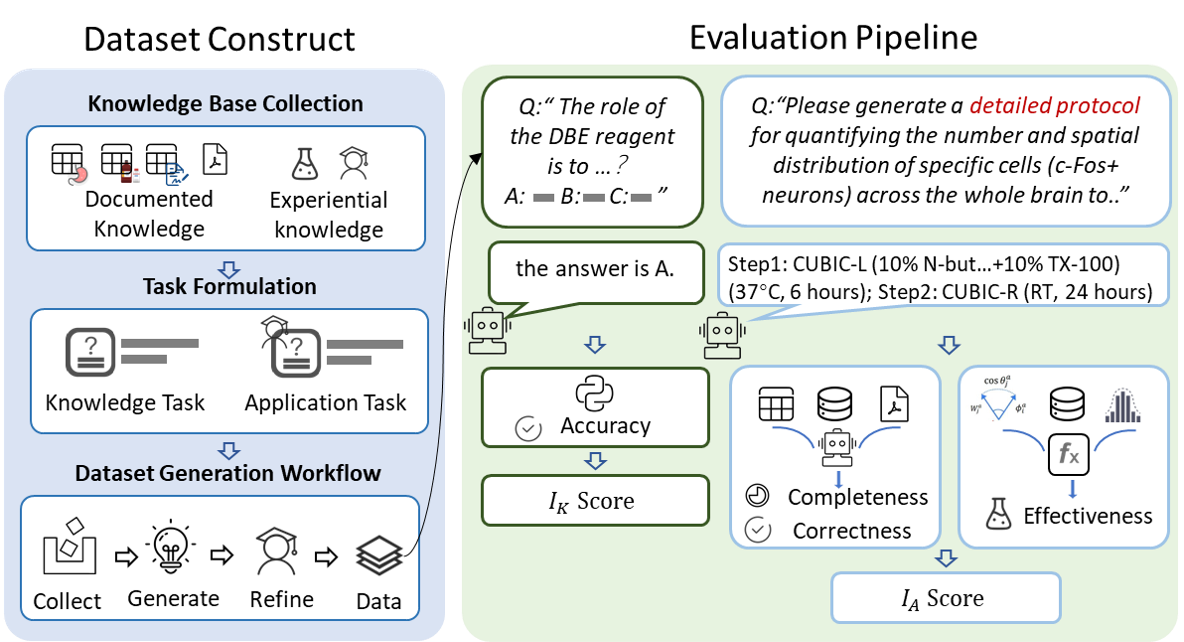
\includegraphics[width=1\linewidth]{figures/overview.png}
    \caption[Overview of the dataset construction and benchmarking pipeline.]{Overview of the dataset construction and benchmarking pipeline. The left panel shows the workflow for formulating domain knowledge into evaluation datasets. The right panel details the evaluation process, scoring knowledge tasks on accuracy ($I_K$) and application tasks on completeness, correctness, and an empirically-grounded effectiveness metric ($f_x$) grounded in experimental confidence intervals to calculate the $I_A$ Score. \par 数据集构建和基准测试管道的概述。左侧面板显示了将领域知识制定为评估数据集的工作流程。右侧面板详细说明了评估过程，对知识任务的准确率（$I_K$）进行评分，并根据基于实验置信区间的完整性、正确性和有效性指标（$f_x$）对应用任务进行评分，以计算 $I_A$ 分数。}
    \label{fig:overview}
\end{figure}

\subsection{Knowledge Base and Task Formulation (知识库与任务制定)}

ClearEval formalizes wet-lab constraints into a computational knowledge system using curated databases of tissue/marker metadata, physicochemical properties, and 20+ mainstream protocols. To mathematically bridge user intent with protocol selection, these constraints are mapped into a 6-dimensional vector space $\mathcal{V} \in[0,1]^6$ (e.g., fluorescence preservation, dye permeability, safety). Grounded in this space, experts defined \textbf{60 core scientific missions} across diverse biological scales to serve as realistic task generation seeds.

ClearEval 利用精选的组织/标记元数据、物理化学性质和 20 多种主流协议的数据库，将湿实验约束形式化为计算知识系统。为了在数学上将用户意图与协议选择联系起来，这些约束被映射到一个 6 维向量空间 $\mathcal{V} \in[0,1]^6$（例如，荧光保留、染料渗透性、安全性）。以此空间为基础，专家定义了跨越不同生物尺度的 \textbf{60 个核心科学任务}，作为现实任务生成的种子。

\subsection{Dataset Generation Workflow (数据集生成工作流)}

ClearEval's pipeline (Fig.~\ref{fig:overview}, bottom left) leverages a DeepSeek-driven RAG system to synthesize 70 decision templates, 60 mission seeds, and 437 literature chunks into task candidates, followed by strict expert validation to eliminate hallucinations. The curated dataset includes \textbf{2,589 Knowledge Tasks (MCQs)} with a strict 8-option format to prevent guessing, and \textbf{253 Application Tasks (OEQs)}. Notably, OEQs eschew static reference answers, providing instead constrained scenarios that are evaluated purely via our automated, empirically-grounded formula pipeline (Fig.~\ref{fig:overview}, right).

ClearEval 的管道（图~\ref{fig:overview}，左下）利用 DeepSeek 驱动的 RAG 系统将 70 个决策模板、60 个任务种子和 437 个文献块合成为任务候选者，随后进行严格的专家验证以消除幻觉。精选的数据集包括 \textbf{2,589 个知识任务（MCQ）}（采用严格的 8 选项格式以防止猜测），以及 \textbf{253 个应用任务（OEQ）}。值得注意的是，OEQ 避开了静态的参考答案，而是提供了受限场景，完全通过我们自动化的、基于经验公式的管道进行评估（图~\ref{fig:overview}，右）。

\section{Evaluation Framework (评估框架)}

To bridge the gap between static knowledge and wet-lab executability, ClearEval introduces a hierarchical evaluation framework (Table~\ref{tab:metrics}). Moving beyond semantic similarity, our Application Index ($I_A$) relies on \textbf{empirically-grounded verification}—modeling experimental confidence intervals for refractive indices and incubation times—as the core of the Effectiveness dimension.

为了弥合静态知识和湿实验可执行性之间的鸿沟，ClearEval 引入了分层评估框架（表~\ref{tab:metrics}）。超越语义相似度，我们的应用指数（$I_A$）依赖于\textbf{基于经验事实的验证}——对折射率和孵育时间的实验置信区间进行建模——作为有效性维度的核心。

\begin{table}[htbp]
    \centering
    \caption{The Hierarchical Metric System of ClearEval. Evaluation spans from static knowledge retrieval to physics-grounded protocol execution.}
    \label{tab:metrics}
    \resizebox{\textwidth}{!}{
    \begin{tabular}{l l l l c} 
        \toprule
        \textbf{Level} & \textbf{Dimension} & \textbf{Sub-Metric} & \textbf{Method} & \textbf{Max} \\
        \midrule
        Knowledge ($I_K$) & Static Retrieval & Accuracy & Deterministic & 100\% \\
        \midrule
        \multirow{9}{*}{Application ($I_A$)} & \multirow{2}{*}{Completeness} & Step Integrity & LLM-Judge & 40\% \\
         & & Param Detail & LLM-Judge & 60\% \\
        \cmidrule{2-5} 
         & \multirow{3}{*}{Correctness} & Sequential Logic & LLM-Judge & 40\% \\
         & & Consistency & LLM-Judge & 20\% \\
         & & Physics Plausibility & LLM-Judge & 40\% \\
        \cmidrule{2-5} 
         & \multirow{4}{*}{Effectiveness} & Method Suitability & Vector Sim. & 30\% \\
         & & Label Compatibility & Rule-Based & 40\% \\
         & & Trans. Validity ($S_{trans}$) & Physics Eq. & 15\% \\
         & & Time Efficiency ($S_{time}$) & Physics Eq. & 15\% \\
        \midrule
        \textbf{Overall} & Expert Score & Harmonic Mean & Aggregation & 100\% \\
        \bottomrule
    \end{tabular}%
    }
\end{table}


\subsection{Knowledge ($I_K$) and Application ($I_A$) Indices (知识与应用指数)}

The \textbf{Knowledge Index ($I_K$)} is the macro-averaged MCQ accuracy across the Tissue \& Marker, Reagent, and Method domains, preventing domain overfitting. 

\textbf{知识指数（$I_K$）} 是跨越组织和标记、试剂以及方法领域的宏平均 MCQ 准确率，防止领域过拟合。

For Open-Ended Questions (OEQs), models generate actionable protocols evaluated on Completeness, Correctness, and Effectiveness. Because a single procedural or chemical violation can ruin a wet-lab experiment, the \textbf{Application Index ($I_A$)} acts as a strict bottleneck, defined as the minimum of these min-max normalized ($[0, 100]$) dimensions: $I_A = \min(\text{Completeness}, \text{Correctness}, \text{Effectiveness})$.

对于开放式问题（OEQ），模型生成可操作的协议，并在完整性、正确性和有效性上进行评估。因为单一的程序或化学违规行为可能会毁掉湿实验，所以\textbf{应用指数（$I_A$）}充当严格的瓶颈，定义为这些最小-最大归一化（$[0, 100]$）维度的最小值：$I_A = \min(\text{完整性}, \text{正确性}, \text{有效性})$。

\subsection{Empirically-Grounded Effectiveness ($E_{score}$) (基于经验事实的有效性)}

This dimension quantitatively verifies protocol feasibility against expert databases and physical constraints, yielding $E_{score} = S_{method} + S_{label} + S_{trans} + S_{time}$:

该维度根据专家数据库和物理约束定量验证协议可行性，得出 $E_{score} = S_{method} + S_{label} + S_{trans} + S_{time}$：

\noindent\textbf{1. Method \& Label Suitability (方法与标签适用性):} 
$S_{method}$ evaluates the cosine similarity between the generated and expert constraint vectors: 
\begin{equation}
S_{method} = 5 \times \text{ReLU}(\cos(\mathbf{v}_{pred}, \mathbf{v}_{ref})). 
\end{equation}
$S_{label}$ is a \textbf{hard constraint}, scoring 0 if any fluorescence quenching risk is detected.

$S_{method}$ 评估生成的约束向量与专家约束向量之间的余弦相似度（见上述等式）。$S_{label}$ 是一个\textbf{硬约束}，如果检测到任何荧光猝灭风险，则得分为 0。

\noindent\textbf{2. Transparency ($S_{trans}$) \& Time Efficiency ($S_{time}$) (透明度与时间效率):} 
To evaluate continuous physical parameters against \textbf{experimental confidence intervals}, we penalize Refractive Index (RI) mismatches and incubation time deviations ($\Delta t$) using Gaussian functions:
\begin{equation}
S_{trans} = 3 \cdot \exp \left( - \frac{(RI_{pred} - RI_{ref})^2}{2\sigma_{RI}^2} \right), \quad
S_{time} = 3 \cdot \exp \left( - \frac{\Delta t^2}{2\tau^2} \right)
\end{equation}
where $\sigma_{RI}$ and $\tau$ are expert-defined tolerance parameters. For $S_{time}$, $\Delta t$ measures the deviation from the physically viable time window $[t_{min}, t_{max}]$.

为了根据\textbf{实验置信区间}评估连续的物理参数，我们使用高斯函数对折射率（RI）不匹配和孵育时间偏差（$\Delta t$）进行惩罚。其中 $\sigma_{RI}$ 和 $\tau$ 是专家定义的公差参数。对于 $S_{time}$，$\Delta t$ 测量偏离物理上可行的时间窗口 $[t_{min}, t_{max}]$ 的程度。

\subsection{Overall Expert Score (整体专家得分)}

To penalize models that memorize facts but fail under practical physical constraints, the \textbf{ClearEval Expert Score} is the harmonic mean: $\text{Score} = 2 I_K I_A / (I_K + I_A)$. Given the bottleneck formulation of $I_A$, a high score demands both broad theoretical recall and strict experimental compliance.

为了惩罚那些能够记住事实但在实际物理约束下失败的模型，\textbf{ClearEval 专家得分}采用调和平均数：$\text{Score} = 2 I_K I_A / (I_K + I_A)$。鉴于 $I_A$ 的瓶颈公式，获得高分既需要广泛的理论回忆，又需要严格的实验合规性。

\section{Experiments (实验)}
\subsection{Models and Settings (模型与设置)}

We benchmarked LLMs across the GPT, Gemini, Claude, DeepSeek, and Qwen families. We set the temperature to $0.0$ for \textbf{Knowledge tasks} to ensure reproducibility, and used official default temperatures for \textbf{Application tasks} to enable reasoning models to fully explore Chain-of-Thought (CoT).

我们对跨越 GPT、Gemini、Claude、DeepSeek 和 Qwen 家族的 LLM 进行了基准测试。我们将\textbf{知识任务}的温度设置为 $0.0$ 以确保可重复性，并为\textbf{应用任务}使用官方默认温度，以使推理模型能够充分探索思维链（CoT）。

\subsection{Main Results: The Knowledge--Execution Gap (主要结果：知识与执行的鸿沟)}

Table~\ref{tab:main_results_total} reveals a stark capability imbalance between static recall and wet-lab execution. This is visually highlighted in Fig.~\ref{fig:radar_chart}: the left panel demonstrates that all evaluated models exhibit uniformly high and tightly clustered proficiency across Knowledge dimensions. In stark contrast, Application Performance (right) is highly erratic. While models generally maintain basic procedural completeness, their trajectories scatter unpredictably and collapse sharply on empirically-constrained Effectiveness metrics (e.g., exact RI matching, viable diffusion times), exposing a severe knowledge--execution gap.

表~\ref{tab:main_results_total} 揭示了静态回忆与湿实验执行之间明显的能力失衡。这一点在图~\ref{fig:radar_chart}中得到了直观的突出显示：左侧面板表明，所有受评估的模型在各个知识维度上都表现出统一的高水平和紧密聚集的熟练度。形成鲜明对比的是，应用表现（右侧）极不稳定。虽然模型通常保持基本的程序完整性，但它们的轨迹不可预测地分散，并在受经验约束的有效性指标（例如精确的 RI 匹配、可行的扩散时间）上急剧崩溃，暴露了严重的知识-执行鸿沟。

\begin{table}[htbp]
    \centering
    \caption[Performance of state-of-the-art models on ClearEval.]{Performance of state-of-the-art models on ClearEval. Evaluation covers Knowledge (MCQ) and Application (OEQ). $I_K$ represents the average of the Knowledge subset, $I_A$ represents the minimum score across the Application subset, and Total is their harmonic mean. \par 最先进模型在 ClearEval 上的表现。评估涵盖知识（MCQ）和应用（OEQ）。$I_K$ 表示知识子集的平均值，$I_A$ 表示应用子集中的最低分，Total 是它们的调和平均数。}
    \label{tab:main_results_total}
    
    \setlength{\tabcolsep}{3pt} 
    \resizebox{\textwidth}{!}{%
    \begin{tabular}{l cccc cccc c} 
        \toprule
        \multirow{2}{*}{\textbf{Models}} & \multicolumn{4}{c}{\textbf{Knowledge (MCQ)}} & \multicolumn{4}{c}{\textbf{Application (OEQ)}} & \multirow{2}{*}{\textbf{Total}} \\
        \cmidrule(lr){2-5} \cmidrule(lr){6-9} 
        & Tissue & Reagent & Method & $I_K$ & Com. & Cor. & Eff. & $I_A$ & \\
        \midrule
        
        \multicolumn{10}{l}{\textit{Proprietary Models}} \\
        \midrule
        GPT-5.2-Fast & \textbf{91.1} & \textbf{88.7} & 93.5 & \textbf{91.1} & \underline{87.1} & \textbf{90.2} & 66.4 & 66.4 & \textbf{76.8} \\
        GPT-5.2-Think & \underline{90.5} & \underline{87.3} & \underline{93.6} & \underline{90.5} & 80.4 & 88.3 & 64.1 & 64.1 & 75.0 \\
        Gemini-3-Flash & 78.7 & 81.8 & 91.1 & 83.9 & 84.6 & 83.3 & 66.4 & 66.4 & 74.1 \\
        Gemini-3-Pro & 88.8 & 77.2 & 86.7 & 84.2 & 81.7 & 84.8 & 66.3 & 66.3 & 74.2 \\
        Claude-4.6-Sonnet & 87.6 & 82.9 & \textbf{94.9} & 88.5 & \textbf{100.0} & 85.8 & 54.2 & 54.2 & 67.2 \\
        
        \midrule
        \multicolumn{10}{l}{\textit{Open-Weight Models}} \\
        \midrule
        GLM-4.7 & 79.3 & 80.2 & 93.5 & 84.3 & 81.9 & \underline{89.6} & \underline{69.0} & \underline{69.0} & 75.9 \\
        GLM-4.7-Think & 78.7 & 70.5 & 90.7 & 80.0 & 78.8 & 87.1 & \textbf{70.3} & \textbf{70.3} & 74.8 \\
        DeepSeek-V3.2 & 79.9 & 77.9 & 91.7 & 83.2 & 84.6 & 76.2 & 62.2 & 62.2 & 71.2 \\
        DeepSeek-V3.2-Think & 85.3 & 83.8 & 93.5 & 87.5 & 75.0 & 71.9 & 62.3 & 62.3 & 72.8 \\
        Qwen3-max & 79.9 & \underline{87.3} & 93.1 & 86.8 & \underline{87.1} & 81.0 & 68.1 & 68.1 & \underline{76.3} \\
        Qwen3-235B-A22B & 77.5 & 81.2 & 89.1 & 82.6 & 64.6 & 67.1 & 53.9 & 53.9 & 65.2 \\
        Qwen3-32B & 73.4 & 78.6 & 89.9 & 80.6 & 56.2 & 46.5 & 55.2 & 46.5 & 59.0 \\
        Qwen3-14B & 73.4 & 77.8 & 88.4 & 79.9 & 48.8 & 39.0 & 54.3 & 39.0 & 52.4 \\

        \bottomrule
    \end{tabular}%
    }
\end{table}

\begin{figure}[htbp]
    \centering
    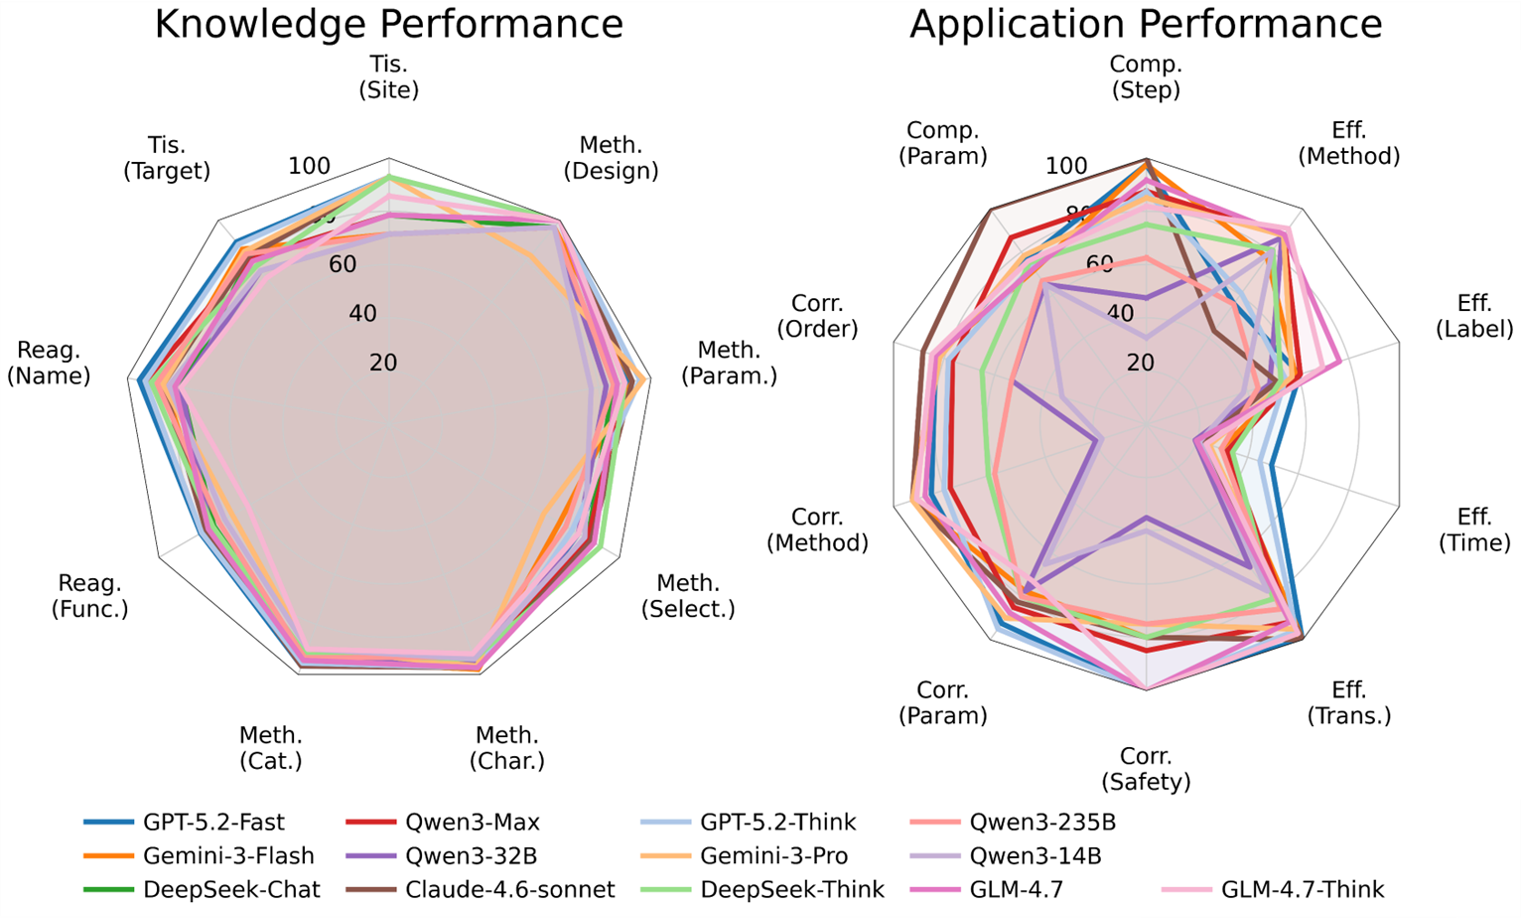
\includegraphics[width=1\linewidth]{figures/combined_radar_chart (6).png}
    \caption[Performance comparison of 13 LLMs on the ClearEval benchmark.]{Performance comparison of 13 LLMs on the ClearEval benchmark. The left panel shows Knowledge Performance ($I_K$) across domain-specific attributes (Tissue, Reagent, Method). The right panel details Application Performance ($I_A$), evaluated on completeness, correctness, and an empirically-grounded effectiveness metric. \par 13 种 LLM 在 ClearEval 基准上的性能比较。左侧面板显示了特定领域属性（组织、试剂、方法）上的知识表现（$I_K$）。右侧面板详细介绍了应用表现（$I_A$），在完整性、正确性和基于经验的有效性指标上进行评估。}
    \label{fig:radar_chart}
\end{figure}

\subsection{Human Alignment of the Automated Metrics (自动化指标的人类对齐度)}

We validated our automated evaluation pipeline against blinded expert judgments on a subset of 260 generated protocols. As shown in Fig.~\ref{fig:alignment}a, alignment varies depending on the underlying evaluation mechanism. Dimensions relying on generic LLM-as-a-judge (Completeness and Correctness) exhibit moderate-to-strong correlations (Pearson $r=0.77$ and $0.69$, respectively), reflecting the inherent instability of LLMs in assessing complex wet-lab logic. Crucially, our core proposed dimension—the empirically-grounded Effectiveness—achieves a strong correlation ($r=0.83$), demonstrating that mathematical constraints provide a far more reliable proxy for expert judgment. 

我们在一个包含 260 个生成协议的子集上，根据盲审专家判断验证了我们的自动评估管道。如图~\ref{fig:alignment}a 所示，对齐情况取决于底层的评估机制。依赖通用“LLM 作为裁判”的维度（完整性和正确性）表现出中等到强的相关性（Pearson $r=0.77$ 和 $0.69$），反映了 LLM 在评估复杂湿实验逻辑时固有的不稳定性。关键的是，我们提出的核心维度——基于经验事实的有效性——实现了很强的相关性（$r=0.83$），这表明数学约束为专家判断提供了可靠得多的代理。

\begin{figure}[htbp]
    \centering
    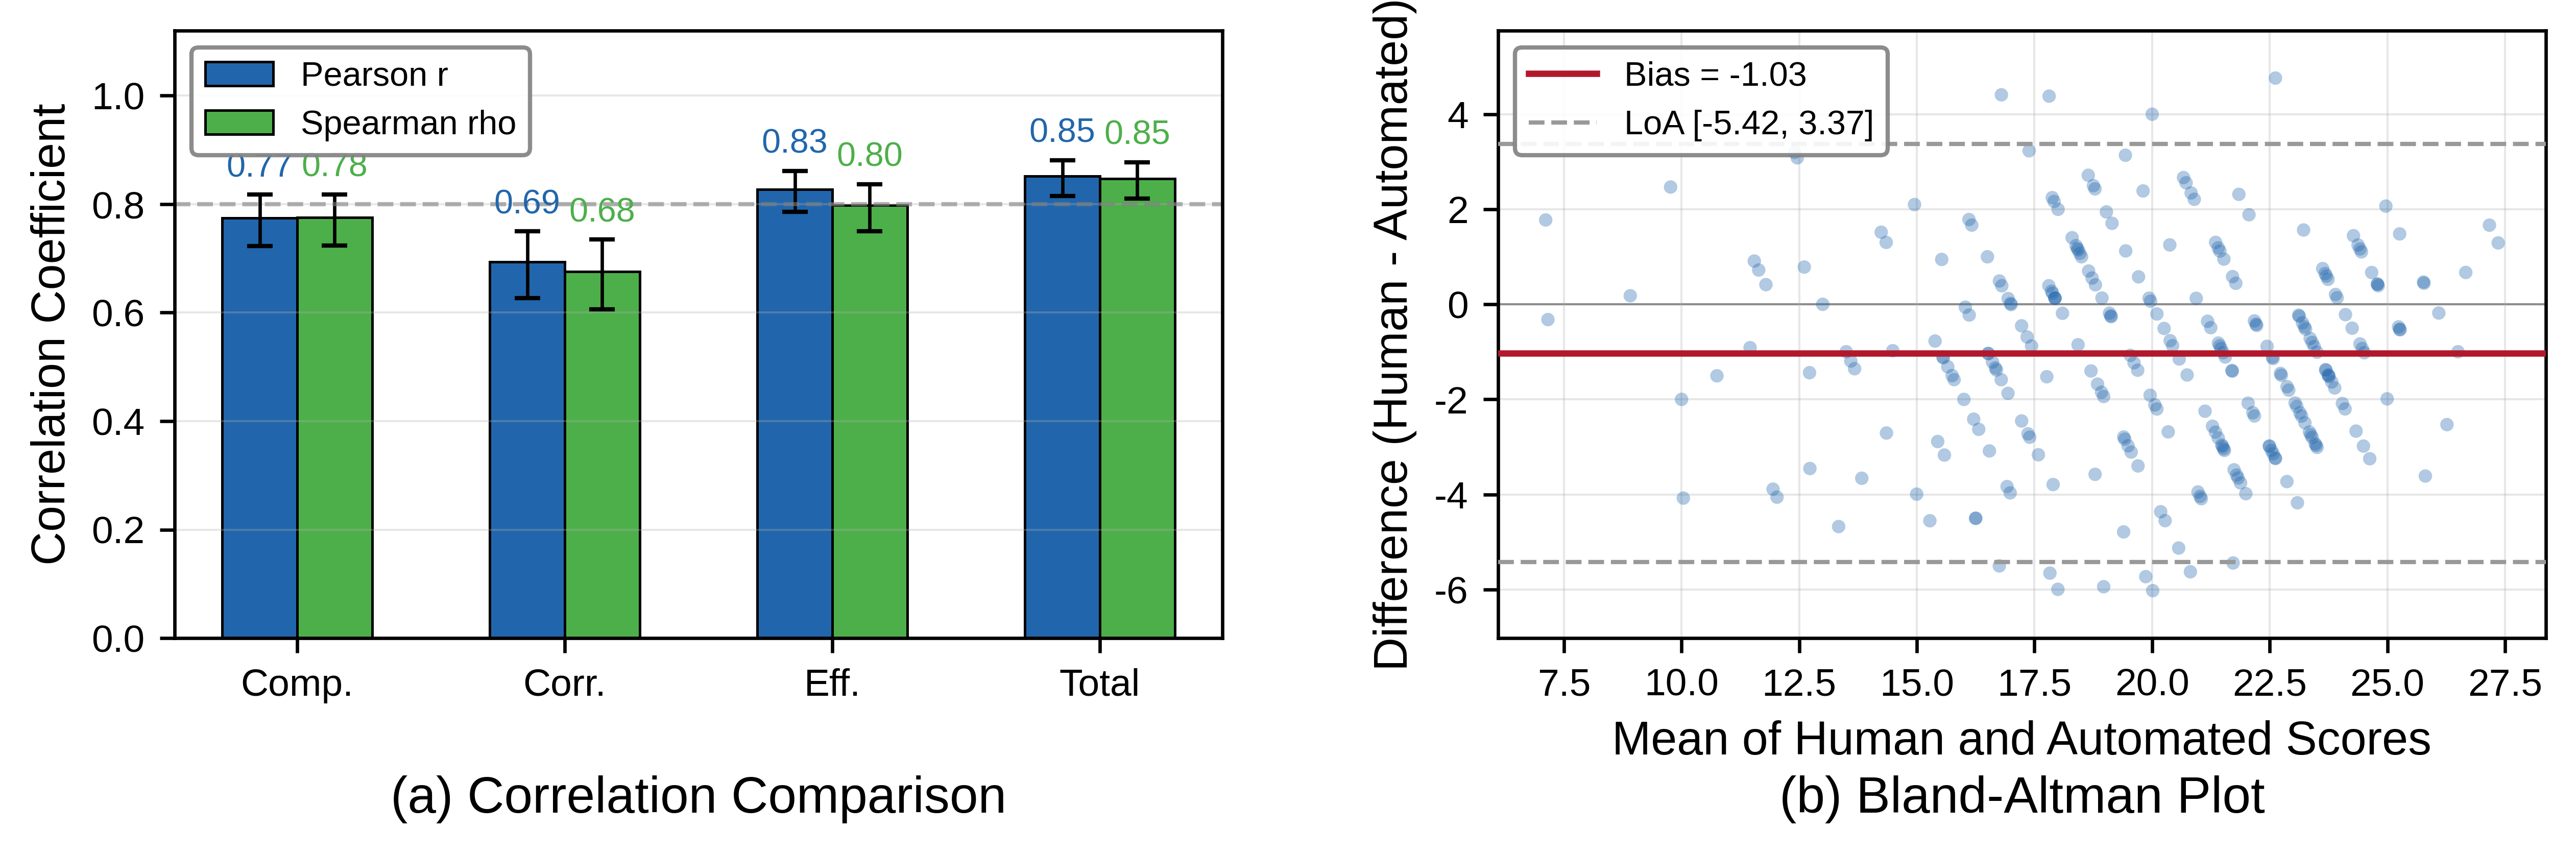
\includegraphics[width=1\linewidth]{figures/conbined_alignment_plots(6).png}
    \caption[Human alignment of automated metrics.]{Human alignment of automated metrics. (a) ClearEval metrics show strong correlation with expert ratings .(b) Bland-Altman plot reveals high absolute agreement with a minimal bias of -1.03. \par 自动化指标的人类对齐度。(a) ClearEval 指标与专家评分显示出强相关性。(b) Bland-Altman 图揭示了极高绝对一致性，偏差仅为 -1.03。}
    \label{fig:alignment}
\end{figure}

\subsection{Fine-Grained Diagnosis: Dissecting the Effectiveness Bottleneck (细粒度诊断：剖析有效性瓶颈)}

To better understand the limitations observed in the Effectiveness metric, we conducted a fine-grained diagnosis to identify specific failure modes. As illustrated in Fig.~\ref{fig:violin_limits}, the overall performance constraint is primarily driven by challenges in Time Efficiency ($S_{time}$) and Label Compatibility ($S_{label}$).

为了更好地理解在有效性指标中观察到的局限性，我们进行了细粒度诊断以识别具体的失败模式。如图~\ref{fig:violin_limits}所示，整体性能的瓶颈主要由时间效率（$S_{time}$）和标签兼容性（$S_{label}$）方面的挑战驱动。

Regarding \textbf{Time Efficiency} ($S_{time}$), while the ground-truth missions span a standard 0--200 hour window, models exhibit notable \textit{scale-insensitivity}. This is visually corroborated by the extended tail distributions in the left panel, where generated incubation times occasionally exceed 800 hours. Further analysis reveals a systematic bias: LLMs tend to underestimate the incubation requirements for large, intact tissues, while simultaneously overestimating the durations for thin sections that require minimal clearing.

关于\textbf{时间效率（$S_{time}$）}，虽然真实的任务跨越标准的 0-200 小时窗口，但模型表现出显著的\textit{尺度不敏感性}。这在左侧面板的延长尾部分布中得到了视觉印证，其中生成的孵育时间偶尔超过 800 小时。进一步分析揭示了系统性偏差：LLM 倾向于低估大型完整组织的孵育要求，同时高估需要最少透明化处理的薄切片的持续时间。

In terms of \textbf{Label Compatibility} ($S_{label}$), the broad distributions spanning the 0--6 score range in the right panel reflect inconsistent performance across different experimental contexts. While models successfully apply high-frequency knowledge—such as the well-documented quenching of fluorescent proteins by organic solvents—they face difficulties in systematically managing the complex chemical compatibility between diverse synthetic dyes (e.g., nuclear or lipid stains) and specific TOC methodologies.

在\textbf{标签兼容性（$S_{label}$）}方面，右侧面板跨越 0-6 分范围的宽泛分布反映了在不同实验背景下不一致的性能。虽然模型成功应用了高频知识——例如记录充分的有机溶剂对荧光蛋白的猝灭——但它们在系统地管理各种合成染料（如核染料或脂质染料）与特定 TOC 方法之间复杂的化学兼容性方面面临困难。

\begin{figure}[htbp]
    \centering
    \makebox[\textwidth][c]{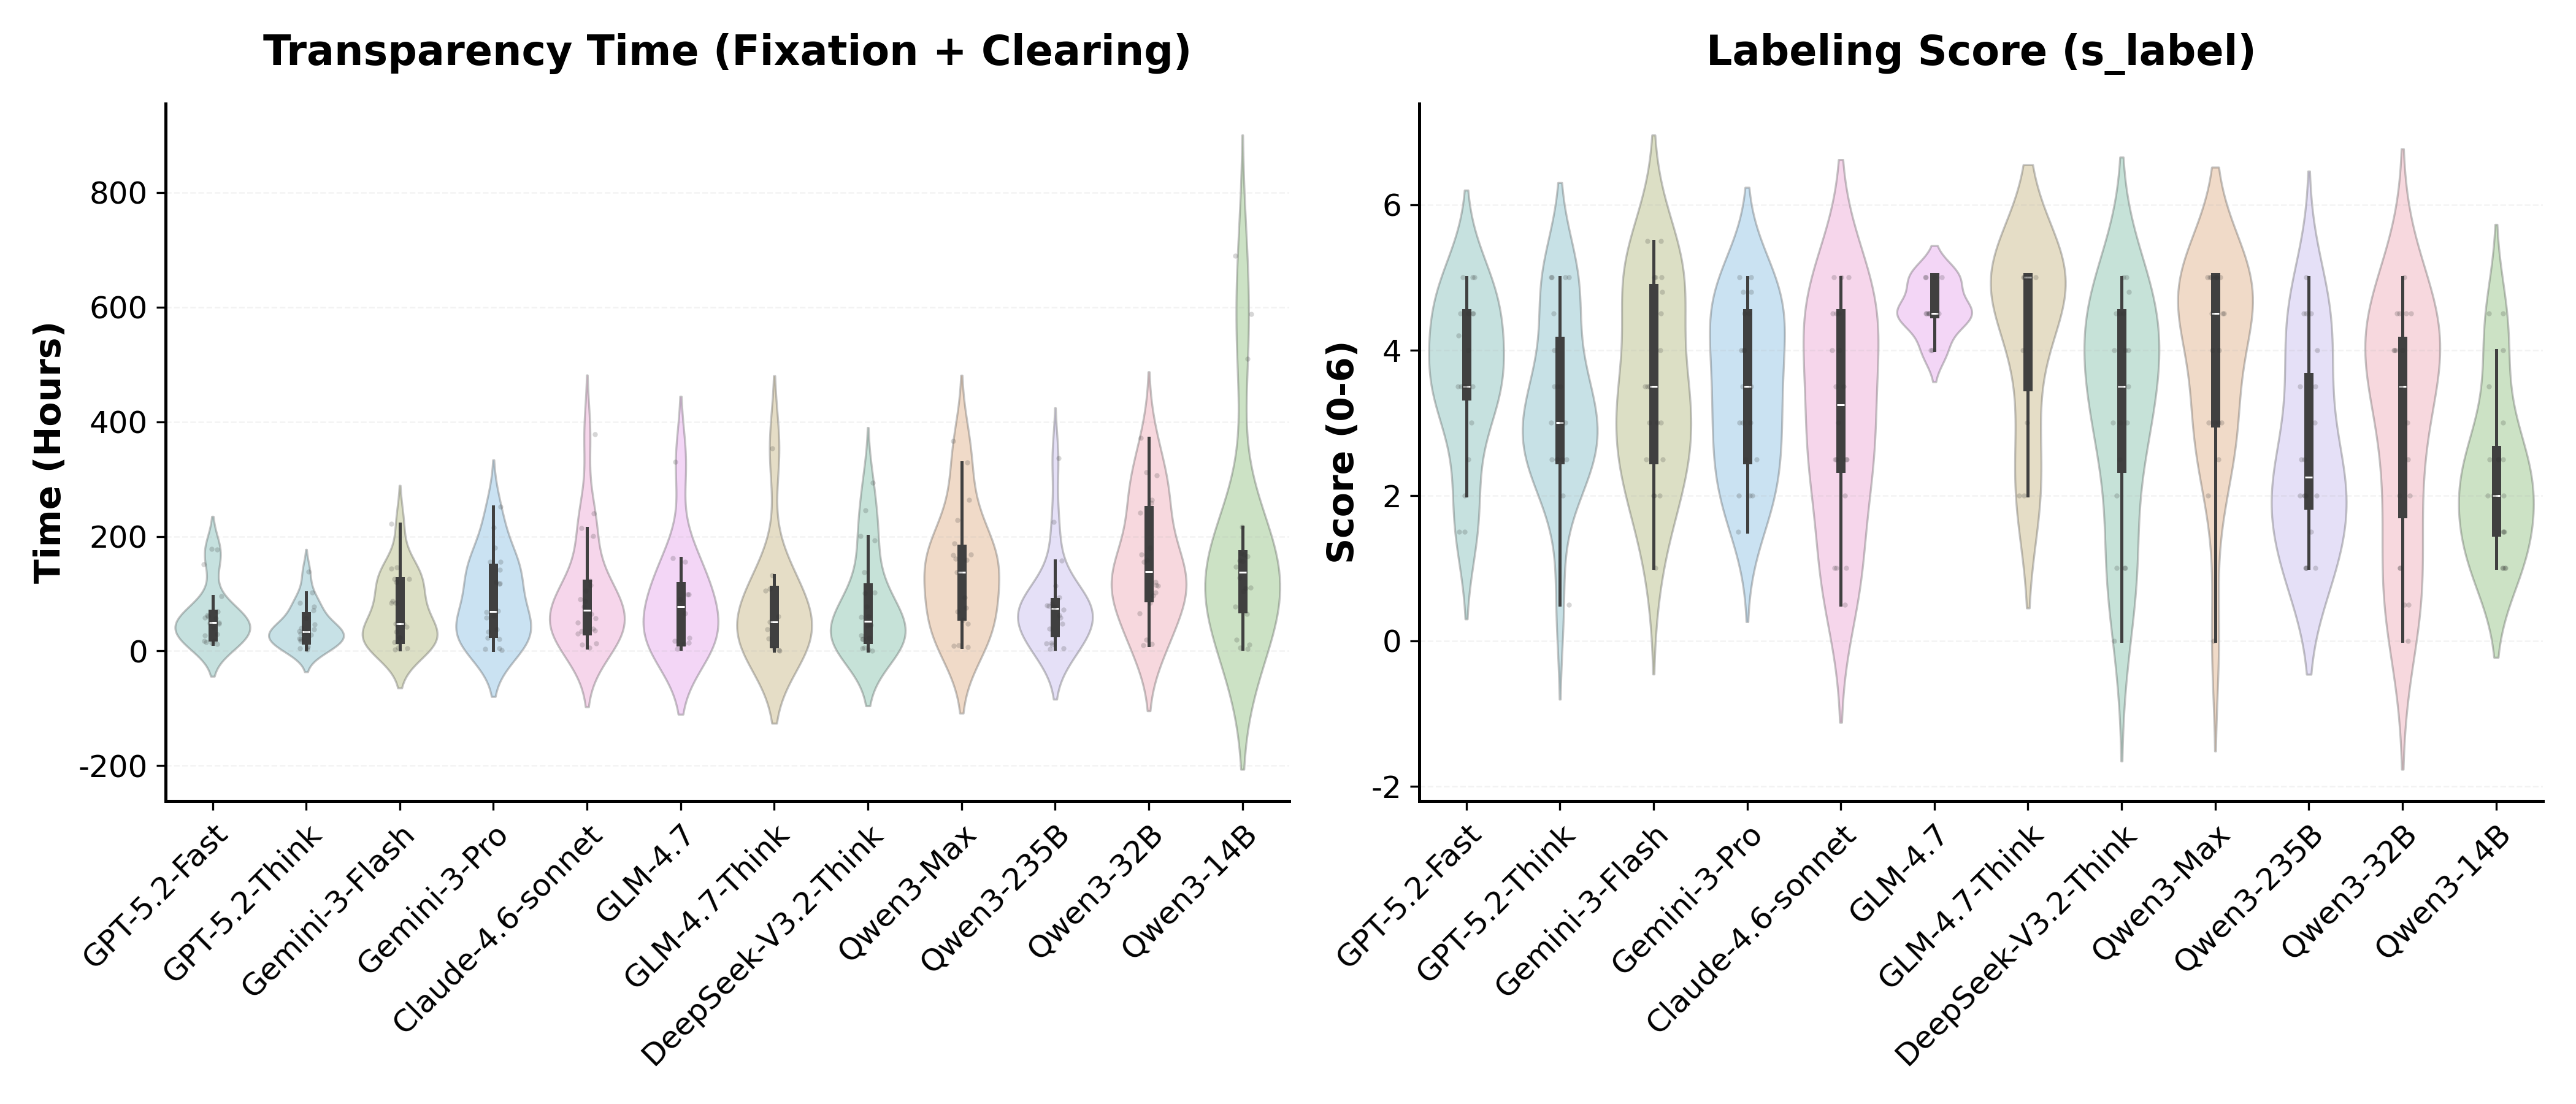
\includegraphics[width=1.2\linewidth]{figures/combined_violin_plots.png}}
    \caption[Performance distribution across different generation strategies.]{Performance distribution across different generation strategies. \par 不同生成策略下的性能分布。}
    \label{fig:violin_limits}
\end{figure}

\section{Discussion and Limitations (讨论与局限性)}

ClearEval identifies that the primary bottleneck in scientific AI is not declarative knowledge retrieval, but the absence of physical grounding. This ``knowledge-action gap'' suggests that for LLMs to truly land in specialized domains, they must transition into \textbf{grounded scientific agents} that internalize physical constraints—such as diffusion kinetics—directly within their reasoning loops. Such agents could serve as the intelligent ``brain'' for closed-loop laboratory instruments, ensuring protocols are functionally executable rather than just linguistically plausible. 

ClearEval 指出，科学 AI 的主要瓶颈不是陈述性知识检索，而是缺乏物理落地。这种“知行鸿沟”表明，为了让 LLM 真正落地于垂直领域，它们必须转变为\textbf{接地的科学智能体}，将扩散动力学等物理约束直接内化到其推理循环中。此类智能体可以充当闭环实验室仪器的智能“大脑”，确保协议在功能上可执行，而不仅仅是语言上合理。

However, our current framework remains a static paradigm. Real-world wet labs involve stochastic variables, such as reagent degradation or tissue heterogeneity, which are difficult to model in silico. Future work will integrate dynamic hardware feedback, enabling autonomous agents to iteratively optimize protocols based on real-time experimental signals. This evolution will transform LLMs from passive consultants into proactive, physics-aware collaborators in the broader AI4Science movement.

然而，我们当前的框架仍然是一个静态范式。现实世界的湿实验涉及随机变量，如试剂降解或组织异质性，这些在计算机模拟中很难建模。未来的工作将整合动态硬件反馈，使自主智能体能够根据实时实验信号迭代优化协议。这种演进将把 LLM 从被动的顾问转变为更广泛的 AI4Science 运动中主动的、具有物理感知的合作者。

\section{Conclusion (结论)}

We presented ClearEval, an expert-level, empirically-grounded benchmark for TOC protocol design with experiment-anchored evaluation.
ClearEval reveals a pronounced knowledge--action gap in current LLMs and provides metrics that align with expert judgments.
We hope ClearEval will facilitate the development of reliable scientific agents for 3D biomedical imaging workflows.

我们提出了 ClearEval，这是一种专家级、基于经验事实的 TOC 协议设计基准测试，并包含基于实验的评估。ClearEval 揭示了当前 LLM 中明显的知行鸿沟，并提供了与专家判断相一致的指标。我们希望 ClearEval 能够促进 3D 生物医学成像工作流中可靠科学智能体的开发。

% ---- Bibliography ----
\bibliographystyle{splncs04}
\bibliography{references}

\end{document}